% uncomment this to get the answer
%\printanswers
%\newtheorem{exercise}[theorem]{Exercise}

\documentclass[a4paper,12pt]{article}%
\usepackage{amsmath}
\usepackage{amsfonts}
\usepackage{amssymb}
\usepackage{graphicx}
\usepackage{hyperref}%
\setcounter{MaxMatrixCols}{30}
%TCIDATA{OutputFilter=latex2.dll}
%TCIDATA{Version=5.50.0.2953}
%TCIDATA{CSTFile=40 LaTeX article.cst}
%TCIDATA{Created=Tuesday, September 15, 2015 18:10:19}
%TCIDATA{LastRevised=Monday, September 27, 2021 17:18:39}
%TCIDATA{<META NAME="GraphicsSave" CONTENT="32">}
%TCIDATA{<META NAME="SaveForMode" CONTENT="1">}
%TCIDATA{BibliographyScheme=Manual}
%TCIDATA{<META NAME="DocumentShell" CONTENT="Standard LaTeX\Blank - Standard LaTeX Article">}
%TCIDATA{Language=American English}
%BeginMSIPreambleData
\providecommand{\U}[1]{\protect\rule{.1in}{.1in}}
%EndMSIPreambleData
\newtheorem{theorem}{Theorem}
\newtheorem{acknowledgement}[theorem]{Acknowledgement}
\newtheorem{algorithm}[theorem]{Algorithm}
\newtheorem{axiom}[theorem]{Axiom}
\newtheorem{case}[theorem]{Case}
\newtheorem{claim}[theorem]{Claim}
\newtheorem{conclusion}[theorem]{Conclusion}
\newtheorem{condition}[theorem]{Condition}
\newtheorem{conjecture}[theorem]{Conjecture}
\newtheorem{corollary}[theorem]{Corollary}
\newtheorem{criterion}[theorem]{Criterion}
\newtheorem{definition}[theorem]{Definition}
\newtheorem{example}[theorem]{Example}
\newtheorem{lemma}[theorem]{Lemma}
\newtheorem{notation}[theorem]{Notation}
\newtheorem{problem}[theorem]{Problem}
\newtheorem{proposition}[theorem]{Proposition}
\newtheorem{remark}[theorem]{Remark}
\newenvironment{proof}[1][Proof]{\noindent\textbf{#1.} }{\ \rule{0.5em}{0.5em}}
\newenvironment{TEUB}[1][Proof]{\noindent\textbf{#1.} }{\ \rule{0.5em}{0.5em}}
\def\NOMDOSSIER{A Production Economy}
\def\NUMERODOSSIER{2}
\def\LECTURENAME{Bayesian Techniques \\ in Macroeconomics}
\def\DIPLOMA{Master - Quantitative Economics, 2$^{nd}$ year}
\def\UNIV{Paris-Dauphine \& PSL Universities}
\def\WEBPAGE{\href{https://vermandel.org/btm/}{https://vermandel.org/btm}}



%\def\LECTURENAME{Bayesian Techniques \\ in Macroeconomics}
\def\DIPLOMA{Master - Quantitative Economics, 2$^{nd}$ year}
\def\UNIV{Paris-Dauphine \& PSL Universities}
\def\WEBPAGE{\href{https://vermandel.org/btm/}{https://vermandel.org/btm}}


% basic  stuff
\usepackage[T1]{fontenc}
\usepackage{lmodern}
\usepackage{graphicx}
\usepackage{color}
\usepackage{xcolor}
\usepackage{hyperref}
\usepackage{eurosym}
\usepackage{natbib}
\usepackage{minted}
\usepackage[most]{tcolorbox}
\usetikzlibrary{calc}
\definecolor{deepblue}{RGB}{0,129,188}
\definecolor{deepblue2}{RGB}{0,26,153}
\definecolor{deepgreen}{RGB}{73,155,202}
\definecolor{mygray}{gray}{0.9}
\definecolor{myblue}{RGB}{0,163,243}

\setlength\parskip{.4em plus 0.1em minus 0.2em}
\setlength{\parindent}{15pt}%

% the page size
\usepackage{geometry}
\geometry{a4paper, top=1.5cm, left=1cm, right=1.0cm, bottom=1.0cm, includehead, includefoot}
\graphicspath{{../},{../../},{/chap1},{/chap2},{/chap3},{/chap4},{/chap5},{/chap6},{../2018_macroeconometrics/}}
\pdfoptionpdfinclusionerrorlevel=0


% TOC programming
\usepackage{tocloft}
\setlength{\cftbeforesecskip}{2pt}
\setcounter{tocdepth}{1} % hide subsection in TOC

%%% BULLET LIST ITEMS
\usepackage{bm}
\newcommand{\localtextbulletone}{\textcolor{deepblue2}{\bm{$\circ$}}}
\renewcommand{\labelitemi}{\localtextbulletone}

% section programming 
\usepackage[calcwidth]{titlesec}
\titleformat{\section}% sectioning command formatted
            {\bfseries\LARGE\color{deepblue2}}% font commands applied to whole
            {\thesection .}% label
            {0.5em}% separation between label and title
            {}% commands before section title
            [{\titlerule[1pt]}]% commands after

\titleformat{\part}% sectioning command formatted
            {\bfseries\large}% font commands applied to whole
            {PARTIE \thepart ~:}% label
            {0.5em}% separation between label and title
            {}% commands before section title
            [{\titlerule[1pt]}]% commands after
			
%\renewcommand{\questionshook}{%
%   \setlength{\labelsep}{6pt}%  --> espace entre la puce et le début du texte
%    \setlength{\leftmargin}{0pt}%  --> espace entre le texte et la marge gauche (sauf pour la premiere ligne)
%    \setlength{\labelwidth}{30pt}% --> taille de la boite contenant la puce. Aligné à droite. Si taille < taille de la puce, la taille de la boite est egale à la taille de la puce
%   \setlength{\listparindent}{\parindent}% --> indentation des paragraphe dans la liste
%    \setlength{\itemindent}{30pt}% --> espace entre la marge et la puce
    %\setlength{\itemsep}{0pt}% --> espace entre les items (auquel s'ajoute \parsep}
%}
%\renewcommand\thequestion{\arabic{question}}
%\renewcommand{\questionlabel}{Question No.~\thequestion.}

%Pdf HYPPERREF STUFF
\hypersetup{
colorlinks=false,
	breaklinks=true,
	plainpages=false,
	%pdftitle={\letitre},
	pdfauthor={University of Paris-Dauphine},
	pdfsubject={},
	pdfcreator={TeX et TXC},
	%pdfstartpage={1},
	%pdfpagemode={FullScreen}
	pdfkeywords={DSGE, Business Cycles},
	pdfborder={0 0 0},
	bookmarksnumbered=true,
	pdfproducer={University Paris-Dauphine},     
	pdfnewwindow=true,          
	colorlinks=true,           
	linkcolor=deepblue,              
	citecolor=deepblue,            
	filecolor=black,          
	urlcolor=deepblue2 
}

% DEALING WITH BOXES
\usepackage{tcolorbox}
\newtcolorbox{mybox}[1]{colback=black!5,colframe=black!40,fonttitle=\bfseries,title=#1,fontlower=\sfdefault}
\newtcolorbox{myconsole}[1]{colback=deepblue!5,colframe=deepblue!40,fonttitle=\bfseries,title=#1,fontlower=\sfdefault}
\newtcolorbox{myresult}[1]{colback=black!5,colframe=deepgreen,fonttitle=\bfseries,title=#1,fontlower=\sfdefault}


%%% EXERCISE BOX
\newtcolorbox[auto counter]{assignment}{
  breakable,
  fonttitle=\bfseries,
  title={Assignment \thetcbcounter}
}
\newtcolorbox[auto counter]{myexercise}[1]{
  skin=enhanced,
  breakable,
  colback=white,
  colframe=gray!30,
  coltitle=black,
  fonttitle=\bfseries,
  leftrule=0.5cm,
  arc=0pt,
  outer arc=0pt,
  title={Exercise \thetcbcounter : #1}
}
\newtcolorbox{definitioniii}[1]{
  skin=enhanced,
  breakable,
  fonttitle=\bfseries,
  colback=white,
  arc=0pt,
  outer arc=0pt,
  title={#1},
  shadow={1mm}{-1mm}{0mm}{fill=gray,opacity=0.5,sharp corners}
}

% DEALING WITH THE EXAM CLASS
%\printanswers % If you want to print answers
% \noprintanswers % If you don't want to print answers
%\addpoints % if you want to count the points
% \noaddpoints % if you don't want to count the points
% Specifies the way question are displayed:
%\qformat{\textbf{Question \thequestion}\hfill}%\quad(\thepoints)\hfill}
%\definecolor{SolutionColor}{rgb}{0.8,0.9,1} % light blue
%\shadedsolutions % defines the style of the solution environment
% \framedsolutions % defines the style of the solution environment
% Defines the title of the solution environment:
%\renewcommand{\solutiontitle}{\noindent\textbf{Solution:}\par\noindent}
%\renewcommand{\questionlabel}{\textbf{~\thequestion)} }

% Table of content
\usepackage{titlesec}
\usepackage{titletoc}
\usepackage[titletoc]{appendix}
\contentsmargin{0pt}
\renewcommand\contentspage{\color{deepblue2}p. \thecontentspage}
\dottedcontents{section}[2.3em]{}{2.3em}{5pt}
\dottedcontents{subsection}[5.5em]{}{3.2em}{5pt}
\renewcommand*\contentsname{\bfseries\color{deepblue2}Content of the Handout}

% FRONT PAGE STUFF
\usepackage{setspace}
\def\FRONTPAGE{%
\begin{picture}(0,0)\unitlength=1cm
%\put (1,0) {\includegraphics[width=7.5em]{PSL.png}}
\put (7.5,-1.4) {
\includegraphics[width=.6\textwidth]{logo-upd.png}}
\end{picture}
\begin{center}
	\color{black!70}
	\ifnum\NUMERODOSSIER<1
		\rule{19cm}{.2pt}\\ \hfill Gauthier Vermandel \textcolor{deepblue2}{\bm{$\circ$}} \textit{gauthier.vermandel@dauphine.psl.eu} \\
		\vspace{2cm}
	\else
		\rule{19cm}{.2pt}\\ \hfill Fall \the\year \\
		\textbf{\large \LECTURENAME }\\
		\vspace{0.5cm}
		\UNIV \\ \DIPLOMA \\
		\vspace{0.5cm}
		Gauthier Vermandel\footnote{Department of Economics, Paris-Dauphine University. Updated slides and codes available on my website: \WEBPAGE.} \hfill \textit{gauthier.vermandel@dauphine.psl.eu} \\
		\rule[0.25cm]{19cm}{.2pt}\\
		\vspace{1cm}
	\fi
	\color{black}
  \ifnum\NUMERODOSSIER<1
	\ifnum\NUMERODOSSIER=0
		\begin{spacing}{1.25}
			\hspace{-.2cm}\textcolor{deepblue2}{\Large\textsc{A Note on}\\\textbf{\LARGE \NOMDOSSIER }}
		\end{spacing}
	 \else
		\begin{spacing}{1.25}
			\hspace{-.2cm}\textcolor{deepblue2}{\textbf{\LARGE \NOMDOSSIER }}
		\end{spacing}	 
	\fi
  \else
	\begin{center}
		\begin{minipage}{0.5\textwidth}
				\centering \textcolor{deepblue2}{ \hspace{-.23cm}\Large \textsc{ Chapter \NUMERODOSSIER }}\\ 
				\vspace{1ex}
		\end{minipage}
		 \\ \vspace{2ex}
		\begin{minipage}{0.65\textwidth}
				\begin{center}
					 \onehalfspacing
					 \textcolor{deepblue2}{ \LARGE\textbf{\NOMDOSSIER }}
					 \doublespacing
				\end{center}
		\end{minipage}
	\end{center}
  \fi
	
	\vspace{0.5cm}
\end{center}
\vspace{0.5cm}
\ifnum\NUMERODOSSIER >-1
	\tableofcontents
\fi

}

% page headers
\ifnum\NUMERODOSSIER >-1
	\usepackage{fancyhdr} %pour modification des pieds de page
	\pagestyle{fancy} % Finally, use the "fancy" page style to implement the FancyHdr headers
	\setlength{\headheight}{14.5pt}
	\fancyhf{}
	\fancyheadoffset{0\textwidth}
	\fancyfoot[C]{\color{black!60} page \thepage}
	\renewcommand{\headrulewidth}{1pt}
	\fancyhead[L]{ \color{deepblue2}\nouppercase{\rightmark}}
\fi




\newcounter{theexercise}
\setcounter{theexercise}{1}
\newenvironment{exercise}
{	
	\vspace{1cm} 
	%\begin{center}\textcolor{black!40}{\rule{6cm}{1px}\\}\end{center} 
	\Large \color{deepblue2} \underline{Exercise \arabic{theexercise}:} 
}
{ 
	\vspace{.5cm}  
	%\begin{center}\textcolor{black!40}{\rule{6cm}{1px}\\}\end{center} 
	\stepcounter{theexercise} 
}


%%%%%%%%%%%%%%%%%%%%%%%%%%%%%%%%%%% NICE COLORBOX
\tcbset{mystyle/.style={
  breakable,
  enhanced,
  outer arc=0pt,
  arc=0pt,
  colframe=myblue,
  colback=myblue!20,
  attach boxed title to top left,
  boxed title style={
    colback=myblue,
    outer arc=0pt,
    arc=0pt,
    top=3pt,
    bottom=3pt,
    },
  fonttitle=\sffamily
  }
}

\newtcolorbox{myobjs}[1][]{
  mystyle,
  title= \large\textsc{Handout Objectives},
  attach boxed title to top center,
  colframe=deepblue,
  colback=white,
   boxed title style={
    colback=deepblue,
    outer arc=2pt,
    arc=2pt,
	top=10pt,bottom=10pt
    },
  outer arc=2pt,
  arc=2pt,
}


\newtcolorbox[auto counter]{myproof}[1][]{
  mystyle,
  colback=white,
  rightrule=0pt,
  toprule=0pt,
  title=Proof \thetcbcounter,
  overlay unbroken and first={
      \path
        let
        \p1=(title.north east),
        \p2=(frame.north east)
        in
        node[anchor=west,font=\sffamily,color=myblue,text width=\x2-\x1] 
        at (title.east) {#1};
  }
}

\newtcolorbox[auto counter]{myMATLAB}[1][]{
  mystyle,
  colframe=deepblue,
  colback=deepblue!0,
  boxed title style={
    colback=deepblue
    },
  title=MATLAB box~\thetcbcounter,
  overlay unbroken and first={
      \path
        let
        \p1=(title.north east),
        \p2=(frame.north east)
        in
        node[anchor=west,font=\sffamily,color=deepblue,text width=\x2-\x1] 
        at (title.east) {#1};
  }
}

\newcommand{\MATLABbox}[1]{
	\vspace{2ex}
	\begin{myMATLAB}[\detokenize{#1}.m]
	%\inputminted[bgcolor=black!10, frame=lines, framesep=8\fboxrule, rulecolor=\color{black!30},framerule=1pt, linenos=true,numbersep=3pt,fontsize=\footnotesize]{matlab}{codes/\detokenize{#1}.m}
	{\centering\includegraphics[width=\textwidth,trim={1cm 0 1cm 0},clip]{codes/\detokenize{#1}.png}}
	\end{myMATLAB}
	\vspace{2ex}
}

\newcommand{\MATLABboxPDF}[1]{
	\vspace{2ex}
	\begin{myMATLAB}[\detokenize{#1}.m]
	%\inputminted[bgcolor=black!10, frame=lines, framesep=8\fboxrule, rulecolor=\color{black!30},framerule=1pt, linenos=true,numbersep=3pt,fontsize=\footnotesize]{matlab}{codes/\detokenize{#1}.m}
	{\centering\includegraphics[width=\textwidth,trim={1cm 0 1cm 0},clip]{codes/\detokenize{#1}.pdf}}
	\end{myMATLAB}
	\vspace{2ex}
}


\newcommand{\MATLABboxNoFig}[1]{
	\vspace{2ex}
	\begin{myMATLAB}[\detokenize{#1}.m!]
	\inputminted[bgcolor=black!10, frame=lines, framesep=8\fboxrule, rulecolor=\color{black!30},framerule=1pt, linenos=true,numbersep=3pt,fontsize=\footnotesize]{matlab}{codes/\detokenize{#1}.m}
	%{\centering\includegraphics[width=\textwidth]{codes/#1.png}}
	\end{myMATLAB}
	\vspace{2ex}
}

%%%% MAKE CODE IN BLUE PLZ
\let\oldtextsf\textsf
\renewcommand{\textsf}[1]{\textcolor{deepblue}{\oldtextsf{#1}}}

\begin{document}
\FRONTPAGE%

%TCIMACRO{\TeXButton{BeginDefinition}{\vspace{4ex}
%\begin{myobjs}}}%
%BeginExpansion
\vspace{4ex}
\begin{myobjs}%
%EndExpansion


\begin{itemize}
\item Solving a rational-expectations model;

\item Linearizing a system of equations;

\item Extend the model.
\end{itemize}

%

%TCIMACRO{\TeXButton{EndDef}{\end{myobjs}}}%
%BeginExpansion
\end{myobjs}%
%EndExpansion


\newpage

\section{A production economy}

Our economy is characterized by a representative household which consumes,
produces goods, accumulates physical capital involved in the production. There
is no labour in this economy as household's labour supply is assumed to be
inelastic to macroeconomic fluctuations while technology does not involve
hours worked. Households are immortal and infinite, the economy is populated
by an infinite number of $j\in\left[  0,1\right]  $ distributed on an unitary contiuum.

The household face the following maximization problem:%
\begin{align*}
&  \max_{C_{jt},K_{jt}}\mathbb{E}_{t}\sum_{\tau=0}^{+\infty}\beta^{\tau}%
\log\left(  C_{jt+\tau}\right) \\
s.t.  &  :C_{jt}+K_{jt}=A_{t}K_{jt-1}^{\alpha}+\left(  1-\delta\right)
K_{jt-1}%
\end{align*}


The budget constraint is actually the result of the comibation of the GDP and
the accumulation of physical capital.\ First, the GDP reads as follows:%
\begin{equation}
C_{jt}+I_{jt}=Y_{jt}. \label{eq hh budget constraint}%
\end{equation}
The total income $Y_{jt}$\ is spent on consumption goods $C_{jt}$ and
investment goods $I_{jt}$.

The law of motion of capital reads as in the \cite{solow1956contribution}'s
model:%
\begin{equation}
I_{jt}=K_{jt}-\left(  1-\delta\right)  K_{jt-1}
\label{eq hh capital law of motion}%
\end{equation}
Investment is determined by the gap between current capital $K_{jt}$\ and
depreciated capital $\left(  1-\delta\right)  K_{jt-1}$. In the latter
expression, the parameter $0\leq\delta\leq1$ denotes the depreciation rate of capital.

The standard Cobb-Douglas technology is determined by:%
\begin{equation}
Y_{jt}=A_{t}K_{jt-1}^{\alpha} \label{eq hh production}%
\end{equation}
where $0<\alpha\leq1$\ is the share of capital involved in the production
process of new goods $Y_{jt}$\ while $A_{t}$\ is a productivity shock which
temporary affects the society's ability to produce goods, it affects all the
households in our economy in the same way. The production combines technology
and capital $K_{jt-1}$ bought in $t-1$ as capital requires one period to be
settled (the so called time-to-build in the RBC literature).\ Concerning the
productivity shock, it is assumed to follow a simple AR(1) process given by:%
\begin{equation}
\log\left(  A_{t}\right)  =\rho_{A}\log\left(  A_{t-1}\right)  +\eta_{t}^{A},
\end{equation}
where $0\leq\rho_{A}<1$ is the autocorrelation coefficient of the shock and
$\eta_{t}^{A}$\ is an innovation distributed normally with zero mean and
finite variance $\sigma_{A}^{2}$ such that $\eta_{t}^{A}\sim\mathcal{N}%
(0,\sigma_{A}^{2})$.%

%TCIMACRO{\TeXButton{BeginExo}{\begin{myexercise}{A production economy}
%\addcontentsline{toc}{section}{Exercise \thetcbcounter}}}%
%BeginExpansion
\begin{myexercise}{A production economy}
\addcontentsline{toc}{section}{Exercise \thetcbcounter}%
%EndExpansion


Consider the production economy model.

\begin{enumerate}
\item Set the Lagrangian problem.

\item Find the first order conditions.\ Get rid off the Lagrangian multiplier
to obtain the Euler equation on physical capital.

\item Write the three equations of the model. Apply aggregation to find the
general equilibrium conditions such that $C_{t}=%
%TCIMACRO{\tint \nolimits_{0}^{1}}%
%BeginExpansion
{\textstyle\int\nolimits_{0}^{1}}
%EndExpansion
C_{jt}$d$j,K_{t}=%
%TCIMACRO{\tint \nolimits_{0}^{1}}%
%BeginExpansion
{\textstyle\int\nolimits_{0}^{1}}
%EndExpansion
K_{jt}$d$j$ and $Y_{t}=%
%TCIMACRO{\tint \nolimits_{0}^{1}}%
%BeginExpansion
{\textstyle\int\nolimits_{0}^{1}}
%EndExpansion
Y_{jt}$d$j$ .\ Find the steady state.

\item Linearize the three equations.
\end{enumerate}

%

%TCIMACRO{\TeXButton{EndExo}{\end{myexercise}}}%
%BeginExpansion
\end{myexercise}%
%EndExpansion


\section{Solving a linear rational-expectations model}

\subsection{A general solution}

Recall that in a general form, a model is a set of nonlinear equations:%

\begin{equation}
\mathbb{E}_{t}\left[  f_{\theta}\left(  x_{t+1},x_{t},x_{t-1},\epsilon
_{t}\right)  \right]  =0, \label{eq non linear system}%
\end{equation}
where $\theta$\ is the set of structural parameters, $x_{t}$\ are endogenous
variables, $\epsilon_{t}$\ are gaussian innovations and $f_{\theta}(\bullet
)$\ is the set of equations.

As disccused in the previous handout, we apply linearization methods to
$f_{\theta}()$ to obtain the set of linear equations:%
\begin{equation}
\mathbb{E}_{t}\left[  \hat{f}_{\theta}\left(  \hat{x}_{t+1},\hat{x}_{t}%
,\hat{x}_{t-1},\epsilon_{t}\right)  \right]  =0 \label{eq: linear system}%
\end{equation}


\textsf{A classification of variables and equations.\ }In order to avoid
singular matrices, we must distinguish between three type of variables: (i)
state variables $\hat{s}_{t}$, (ii) jump variables $\hat{\jmath}_{t}$ and
(iii) exogenous shock processes $\hat{z}_{t}$.\footnote{Note that Dynare has a
different classification for endogenous variables as exogenous variables are
also considered as state ones.} State variables feature persistence and are
determined by other variables, they are key in shaping the propagation
mechanism of a business cycle model. Unlike state variables, jump variables
don't feature some pesistence.\ Finally, exogenous shocks are simply
self-determined variables as they don't depend on any other variables. Note
that Dynare automatically detects states and jump variables and reports their
respective numbers in the command window of MATLAB.

Given the previous dichotomy across endogenous variables $\hat{x}_{t}=[\hat
{s}_{t},\hat{z}_{t},\hat{\jmath}_{t}]^{\prime}$, we also must distinguish
between three types of equations in our linearized model $\hat{f}_{\theta}()$:
\
\begin{align}
0  &  =E_{t}\left[
\begin{array}
[c]{cccc}%
A_{0}\hat{s}_{t}+ & A_{-1}\hat{s}_{t-1}+ & B_{0}\hat{\jmath}_{t}+ & C_{0}z_{t}%
\end{array}
\right]  ,\label{eq: sys1}\\
0  &  =E_{t}\left[
\begin{array}
[c]{ccccccc}%
D_{1}\hat{s}_{t+1}+ & D_{0}\hat{s}_{t}+ & D_{-1}\hat{s}_{t-1}+ & M_{1}%
\hat{\jmath}_{t+1}+ & M_{0}\hat{\jmath}_{t}+ & L_{1}\hat{z}_{t+1}+ & L_{0}%
\hat{z}_{t}%
\end{array}
\right]  ,\label{eq: sys2}\\
\ \hat{z}_{t}  &  =Z\hat{z}_{t-1}+\epsilon_{t}\text{, }\epsilon_{t}%
\sim\mathcal{N}(0,Q).\ \label{eq: sys3}%
\end{align}
The first set of equations stacks equations with no expectation terms, the
second set of equations must feature at least one forward looking variable,
and the last set of equation are exogenous shock processes.

\textsf{The functional form of the solution.\ }We are looking for a recursive
solution of our model:%
\begin{equation}
\hat{x}_{t}=F\hat{x}_{t-1}+G\hat{z}_{t},
\end{equation}
where $F$\ and $G$ are yet two unknown matrices. Note that this solution must
hold for any transitions of $\hat{x}$ either from $t+1\rightarrow t$ or
$t\rightarrow t-1$ consistently with our linearized system $\hat{f}_{\theta
}()$.\ Using our classification, this solution can be expressed as two
separate processes:%
\begin{equation}
\left[
\begin{array}
[c]{c}%
\hat{s}_{t}\\
\hat{\jmath}_{t}%
\end{array}
\right]  =\left[
\begin{array}
[c]{cc}%
F_{s} & 0_{n_{j}}\\
F_{j} & 0_{n_{j}}%
\end{array}
\right]  \left[
\begin{array}
[c]{c}%
\hat{s}_{t-1}\\
\hat{\jmath}_{t-1}%
\end{array}
\right]  +\left[
\begin{array}
[c]{c}%
G_{s}\\
G_{j}%
\end{array}
\right]  \hat{z}_{t}%
\end{equation}


The unknown in the previous system are matrices $F_{s}$, $F_{j}$,\ $G_{s}$ and
$G_{j}$. Another way to present the solution reads as follows:%
\begin{align}
\hat{s}_{t}  &  =F_{s}\hat{s}_{t-1}+G_{s}\hat{z}_{t},\label{eq PQ1}\\
\hat{\jmath}_{t}  &  =F_{j}\hat{s}_{t-1}+G_{j}\hat{z}_{t}. \label{eq PQ2}%
\end{align}


\textsf{Solution of the system. }To obtain the unknowns of our transition
equation, consider our first set of equations in \autoref{eq: sys1}. We must
use equations (\ref{eq PQ1}-\ref{eq PQ2}) to replace $\hat{s}_{t}$\ and
$\hat{\jmath}_{t}$ as follows: \ \
\begin{align*}
0  &  =%
\begin{array}
[c]{cccc}%
A_{0}\hat{s}_{t}+ & A_{-1}\hat{s}_{t-1}+ & B_{0}\hat{\jmath}_{t}+ & C_{0}z_{t}%
\end{array}
\\
0  &  =%
\begin{array}
[c]{cccc}%
A_{0}\left(  F_{s}\hat{s}_{t-1}+G_{s}z_{t}\right)  + & A_{-1}\hat{s}_{t-1}+ &
B_{0}\left(  F_{j}\hat{s}_{t-1}+G_{j}z_{t}\right)  + & C_{0}z_{t}%
\end{array}
\\
0  &  =\underset{\text{condition (1)}}{\underbrace{\left[  A_{0}F_{s}%
+A_{-1}+B_{0}F_{j}\right]  }}\hat{s}_{t-1}+\underset{\text{condition (2)}%
}{\underbrace{\left[  A_{0}G_{s}+B_{0}G_{j}+C_{0}\right]  }}z_{t}%
\end{align*}
We do exactly the same for the second set of equation in stacked in
\autoref{eq: sys2} to obtain:%

\begin{multline*}
0=\underset{\text{condition (3)}}{\underbrace{\left[  D_{1}\left(
F_{s}\right)  ^{2}+D_{0}F_{s}+M_{1}F_{j}G_{s}+D_{-1}+M_{0}F_{j}\right]  }}%
\hat{s}_{t-1}\\
+\underset{\text{condition (4)}}{\underbrace{\left[  D_{1}F_{s}G_{s}%
+D_{0}G_{s}+M_{1}F_{j}G_{s}+M_{0}G_{j}+D_{1}G_{s}Z+M_{1}G_{j}Z+L_{1}%
Z+L_{0}\right]  }}\hat{z}_{t},
\end{multline*}
Note that we have 4 conditions and four unknown, so we should theoretically be
able to derive the value $F_{s}$, $F_{j}$\ and\ $G_{s}$, $G_{j}$. However in
practice, it's not as obvious because condition (3) is a quadratic matrix
equation problem of the form $AX^{2}+BX+\ C=0$. There are two implications
from this quadratic problem:

\begin{enumerate}
\item \ Obtaining the closed-form expression of $\left(  F_{s}\right)  ^{2}$
is rather difficult, but fortunately \cite{uhlig1995toolkit} provides a
solution in his Theorem 3.\ In addition, Dynare has also its own routine to
solve linear model (based on the Schur decomposition).\ 

\item The quadractic form of the equations allows multiple roots, that is to
say there are two matrices $F_{s}$\ that solves our models.\ So our economy
can possibly follow two different trajectories for the same system of
equation. In pratice, one of these two path is unstable, so macroeconomists
typically check the eigen values of both systems and pick the stable root.
Note that Dynare also automatically picks the stable roots and provide to the
user the eigen values of the system.\ Finally, a last remark, you may have
noticed that if $D_{1}$\ is all of zeros, then the quadractic problems disappears.
\end{enumerate}

Let us assume that we have followed carefully theorem (3) from
\cite{uhlig1995toolkit}, which allowed us to solve the quadractic matrix
equation problem and pick the stable root of the system.\ If $S_{s}$ is known,
then condition (1) allows us to find $F_{j}$\ as follows:
\begin{equation}
F_{j}=-\left(  B_{0}\right)  ^{-1}\left(  A_{0}F_{s}+A_{-1}\right)
\end{equation}
Mixing both condition (2) and (4) allows to pin down the two remaining unknown
matrices:%
\begin{align}
G_{j}  &  =\left(  M_{0}+M_{1}Z\right)  ^{-1}\left[  \left(  A_{0}\right)
^{-1}\left(  B_{0}G_{j}+C_{0}\right)  \left(  D_{1}F_{s}+D_{0}+M_{1}%
F_{j}+D_{1}Z\right)  -\left(  L_{1}Z+L_{0}\right)  \right]  ,\\
G_{s}  &  =-\left(  A_{0}\right)  ^{-1}\left(  B_{0}G_{j}+C_{0}\right)  .
\end{align}
Prior the spread of Dynare within the profession, macroeconomists used to
linearize their model's equations, to find the steady state, and to fill
matrices in \autoref{eq: sys1}-\ref{eq: sys2}-\ref{eq: sys3} to get the
model's dynamics.\ Changing a single equation would imply to update all the
equations. Dynare really simplified the problem by automating the
linearization of equations, filling the matrices, find the solution, pick the
stable root, plot the IRF, and get second moment statistics. \ Note also that
the number of elements in matrices increases exponentially in the number of
variables, this is referred to as \textsf{the curse of dimensionality}. So,
most of DSGE\ models were rather small prior the use of Dynare.

\textsf{Dynare forumulation.\ }Note that Dynare consider exogenous shock
processes as state variables, replacing $\hat{z}_{t}$\ into the system, we
obtain:
\begin{equation}
\left[
\begin{array}
[c]{c}%
\hat{s}_{t}\\
\hat{\jmath}_{t}%
\end{array}
\right]  =\left[
\begin{array}
[c]{ccc}%
F_{s} & 0_{n_{z}} & 0_{n_{j}}\\
F_{j} & 0_{n_{z}} & 0_{n_{j}}%
\end{array}
\right]  \left[
\begin{array}
[c]{c}%
\hat{s}_{t-1}\\
\hat{\jmath}_{t-1}%
\end{array}
\right]  +\left[
\begin{array}
[c]{c}%
G_{s}\\
G_{j}%
\end{array}
\right]  Z\hat{z}_{t-1}+\left[
\begin{array}
[c]{c}%
G_{s}\\
G_{j}%
\end{array}
\right]  \epsilon_{t}\text{,}%
\end{equation}
which is formulated in Dynare as$:$%
\begin{equation}
\left[
\begin{array}
[c]{c}%
\hat{s}_{t}\\
\hat{z}_{t}\\
\hat{\jmath}_{t}%
\end{array}
\right]  =\left[
\begin{array}
[c]{ccc}%
F_{s} & G_{s}Z & 0_{n_{j}}\\
0_{n_{s}} & Z & 0_{n_{j}}\\
F_{j} & G_{j}Z & 0_{n_{j}}%
\end{array}
\right]  \left[
\begin{array}
[c]{c}%
\hat{s}_{t-1}\\
\hat{z}_{t-1}\\
\hat{\jmath}_{t-1}%
\end{array}
\right]  +\left[
\begin{array}
[c]{c}%
G_{s}\\
1_{n_{z}}\\
G_{j}%
\end{array}
\right]  \epsilon_{t}%
\end{equation}
Or equivalently to the initial form of the policy rule:%
\begin{equation}
\hat{x}_{t}=F\hat{x}_{t-1}+G\epsilon_{t}, \label{eq PQ rule}%
\end{equation}


\subsection{An application to the production economy}

Let's go back to a production economy linearized as follows:%
\begin{align*}
-\hat{k}_{t}+k_{1}\hat{a}_{t}+k_{2}\hat{k}_{t-1}-k_{3}\hat{c}_{t}  &  =0\\
-\hat{c}_{t}+\hat{c}_{t+1}-c_{1}\hat{a}_{t+1}-c_{2}\hat{k}_{t}  &  =0\\
-\hat{a}_{t}+\rho_{A}\hat{a}_{t-1}+\eta_{t}^{A}  &  =0
\end{align*}
where $k_{1}=K^{\alpha-1}\rho_{A}$, $k_{2}=K^{\alpha-1}\alpha+\left(
1-\delta\right)  $, $k_{3}=\bar{C}/\bar{K}$ , $c_{1}=\beta\alpha\bar
{K}^{\alpha-1}$, $c_{2}=\beta\alpha\bar{K}^{\alpha-1}\left(  \alpha-1\right)
$ and$\ E_{t}\hat{a}_{t+1}=\rho_{A}\hat{a}_{t}$. Note that this system is
referred to as \autoref{eq: linear system} in the previous subsection.

Our solution reads as:%
\begin{align}
\hat{c}_{t}  &  =F_{c}\hat{k}_{t-1}+G_{c}\hat{a}_{t},\label{eq PQc}\\
\hat{k}_{t}  &  =F_{k}\hat{k}_{t-1}+G_{k}\hat{a}_{t}.
\end{align}
where $F_{c}$, $F_{c}$, $G_{k}$, $G_{k}$ are yet unknown that we must find. To
obtain these unknowns, we must inject these two equations in the previous
system.\ Let us start with the first equation:
\begin{align*}
-\hat{k}_{t}+k_{1}\hat{a}_{t}+k_{2}\hat{k}_{t-1}-k_{3}\hat{c}_{t}  &  =0,\\
-\left(  F_{k}\hat{k}_{t-1}+G_{k}\hat{a}_{t}\right)  +k_{1}\hat{a}_{t}%
+k_{2}\hat{k}_{t-1}-k_{3}\left(  F_{c}\hat{k}_{t-1}+G_{c}\hat{a}_{t}\right)
&  =0,\\
\underset{\text{condition (1)}}{\underbrace{\left[  k_{2}-k_{3}F_{c}%
-F_{k}\right]  }}\hat{k}_{t-1}+\underset{\text{condition (2)}}{\underbrace
{\left[  k_{1}-k_{3}G_{c}-G_{k}\right]  }}\hat{a}_{t}  &  =0.
\end{align*}%
\begin{align*}
-F_{k}\hat{k}_{t-1}-G_{k}\hat{a}_{t}+k_{1}\hat{a}_{t}+k_{2}\hat{k}_{t-1}%
-k_{3}F_{c}\hat{k}_{t-1}-k_{3}G_{c}\hat{a}_{t}  &  =0,\\
\left(  -F_{k}+k_{2}-k_{3}F_{c}\right)  \hat{k}_{t-1}+\left(  k_{1}-k_{3}%
G_{c}-G_{k}\right)  \hat{a}_{t}  &  =0,
\end{align*}


Note that we must keep injecting these equations until we obtain a system made
of $\hat{k}_{t-1}$ and $\hat{a}_{t}$. Following those steps, we obtain two
conditions on parameters. For the second equation, we do exactly the same as
the previous equation to obtain a system with variables ($\hat{k}_{t-1}%
,\hat{a}_{t}$):
\begin{align*}
-\hat{c}_{t}+\hat{c}_{t+1}-c_{1}\hat{a}_{t+1}-c_{2}\hat{k}_{t}  &  =0,\\
-\hat{c}_{t}+F_{c}\hat{k}_{t}+G_{c}\hat{a}_{t+1}-c_{1}\hat{a}_{t+1}-c_{2}%
\hat{k}_{t}  &  =0,\\
-\hat{c}_{t}+\left(  F_{c}-c_{2}\right)  \hat{k}_{t}+\rho\left(  G_{c}%
-c_{1}\right)  \hat{a}_{t}  &  =0,\\
F_{c}\hat{k}_{t-1}-G_{c}\hat{a}_{t}+\left(  F_{c}-c_{2}\right)  \left(
F_{k}\hat{k}_{t-1}+G_{k}\hat{a}_{t}\right)  +\rho\left(  G_{c}-c_{1}\right)
\hat{a}_{t}  &  =0,\\
\underset{\text{condition (3)}}{\underbrace{\left[  -F_{c}+\left(  F_{c}%
-c_{2}\right)  F_{k}\right]  }}\hat{k}_{t-1}+\underset{\text{condition (4)}%
}{\underbrace{\left[  \left(  F_{c}-c_{2}\right)  G_{k}+\rho\left(
G_{c}-c_{1}\right)  -G_{c}\right]  }}\hat{a}_{t}  &  =0.
\end{align*}
If we find the values of $F_{c}$, $G_{c}$, $F_{k}$, $G_{k}$ that satisfies
conditions (1-4), then we have found the solution of our model. Consider these
four conditions:%
\begin{align*}
\text{condition (1)}  &  :0=k_{2}-k_{3}F_{c}-F_{k}\\
\text{condition (2)}  &  :0=k_{1}-k_{3}G_{c}-G_{k}\\
\text{condition (3)}  &  :0=F_{c}+\left(  F_{c}-c_{2}\right)  F_{k}\\
\text{condition (4)}  &  :0=-G_{c}+\left(  F_{c}-c_{2}\right)  G_{k}%
+\rho\left(  G_{c}-c_{1}\right)
\end{align*}
Combining condition (1) and (3), we obtain the following problem:%
\[
-k_{3}F_{c}^{2}+\left(  k_{3}c_{2}-1+k_{2}\right)  F_{c}-k_{2}c_{2}=0.
\]
Note that this problem has two roots, the usual practice in macroeconomics is
to pick the 'stable' root of the sytem, ie
%TCIMACRO{\TEXTsymbol{\vert}}%
%BeginExpansion
$\vert$%
%EndExpansion
$F_{c}|<1$. Based on the stable root, we can get the rest of the unknown
recursively as follows:
\begin{align*}
F_{k}  &  =k_{2}-k_{3}F_{c}\\
G_{c}  &  =\frac{\left(  F_{c}-c_{2}\right)  k_{1}-\rho c_{1}}{\left(
F_{c}-c_{2}\right)  k_{3}+\left(  1-\rho\right)  }\\
G_{k}  &  =k_{1}-k_{3}G_{c}%
\end{align*}
To get a presentation of the solution close to the one of Dynare, the problem
can be recast as follows%
\begin{equation}
\left[
\begin{array}
[c]{c}%
\hat{k}_{t}\\
\hat{a}_{t}\\
\hat{c}_{t}%
\end{array}
\right]  =\left[
\begin{array}
[c]{ccc}%
F_{k} & G_{k}\rho_{A} & 0\\
0 & \rho_{A} & 0\\
F_{c} & G_{c}\rho_{A} & 0
\end{array}
\right]  \left[
\begin{array}
[c]{c}%
\hat{k}_{t-1}\\
\hat{a}_{t-1}\\
\hat{c}_{t-1}%
\end{array}
\right]  +\left[
\begin{array}
[c]{c}%
G_{k}\\
1\\
G_{c}%
\end{array}
\right]  \epsilon_{t}. \label{eq PQ full}%
\end{equation}
Which we will write as in the next section:%
\begin{equation}
x_{t}=Fx_{t-1}+G\epsilon_{t}, \label{eq PQ compact}%
\end{equation}
where $x_{t}=[\hat{k}_{t},\hat{a}_{t},\hat{c}_{t}]^{\prime}$.%

%TCIMACRO{\TeXButton{MATLABbox}{\MATLABboxPDF{compareRBC}}}%
%BeginExpansion
\MATLABboxPDF{compareRBC}%
%EndExpansion


\newpage

\section{Dynare Programming}

We want to write the model into a form Dynare can interpret. In the first part
of the Dynare code, we need to define the endogenous variables which appear in
the model. There are three equations, so we have three variables: $c_{t}$,
$k_{t}$ and $a_{t}$. The syntax for writing this in Dynare is \textsf{var
[variable1 variable2, ... ]}; with the line ended by a semicolumn. For our
model, we write:%

%TCIMACRO{\TeXButton{Minted}{\vspace{1ex}
%\begin{minted}[bgcolor=mygray,breaklines,linenos]{matlab}
%var k a c;
%\end{minted}
%\vspace{1ex}}}%
%BeginExpansion
\vspace{1ex}
\begin{minted}[bgcolor=mygray,breaklines,linenos]{matlab}
var k a c;
\end{minted}
\vspace{1ex}%
%EndExpansion


Next we write the parameters of the model. In our model, there are four
structural parameters ($\alpha$, $\beta$, $\delta$ and $\rho_{A}$) plus two
steady state variables present in the linear model ($\bar{C}$ and $\bar{K}$),
giving six parameters to declare. The syntax for writing this in Dynare is
\textsf{parameters parameter1 parameter2, ... ;} with the line ended by a
semicolumn. Here we note:%

%TCIMACRO{\TeXButton{Minted}{\vspace{1ex}
%\begin{minted}[bgcolor=mygray,breaklines,linenos]{matlab}
%parameters  alpha beta delta rho_A Css Kss;
%\end{minted}
%\vspace{1ex}}}%
%BeginExpansion
\vspace{1ex}
\begin{minted}[bgcolor=mygray,breaklines,linenos]{matlab}
parameters  alpha beta delta rho_A Css Kss;
\end{minted}
\vspace{1ex}%
%EndExpansion


Next, we write the exogenous variables in the model. We only have one:
$\eta_{t}$. The syntax for writing this in Dynare is\textsf{ varexo variable1
variable2, ... ;} with the line ended by a semicolumn. For our set-up, we write:%

%TCIMACRO{\TeXButton{Minted}{\vspace{1ex}
%\begin{minted}[bgcolor=mygray,breaklines,linenos]{matlab}
%varexo e_a;
%\end{minted}
%\vspace{1ex}}}%
%BeginExpansion
\vspace{1ex}
\begin{minted}[bgcolor=mygray,breaklines,linenos]{matlab}
varexo e_a;
\end{minted}
\vspace{1ex}%
%EndExpansion


Finally, we give the parameters values using our calibration
in\ \autoref{table workspace}. The syntax for giving parameters values is
\textsf{parameter = value;} which is similar to normal Matlab code. We write:%

%TCIMACRO{\TeXButton{Minted}{\vspace{1ex}
%\begin{minted}[bgcolor=mygray,breaklines,linenos]{matlab}
%alpha	= 0.40;		
%beta    	= 0.99;		
%delta    	= 0.025;		
%rho_A	= 0.95;		
%Kss	= ((1/beta-(1-delta))/alpha)^(1/(alpha-1));
%Css	= Kss^alpha - delta*Kss;
%\end{minted}
%\vspace{1ex}}}%
%BeginExpansion
\vspace{1ex}
\begin{minted}[bgcolor=mygray,breaklines,linenos]{matlab}
alpha	= 0.40;		
beta    	= 0.99;		
delta    	= 0.025;		
rho_A	= 0.95;		
Kss	= ((1/beta-(1-delta))/alpha)^(1/(alpha-1));
Css	= Kss^alpha - delta*Kss;
\end{minted}
\vspace{1ex}%
%EndExpansion


We now write the equations of the linearised model. Those equations are
usually written in the same way as they appear in the paper. The equation
section starts with \textsf{model (linear);} and ends with \textsf{end;}%
.\footnote{Note that the tag \textsf{model (linear);} includes the option
'linear' because the model is already linearized.\ For fully non-linear model,
just write \textsf{model ;}.} A few syntax considerations:

\begin{enumerate}
\item Variables which are multiplied (divided) by a parameter are separated by
the parameter by the symbol * (/).

\item Contemporaneous variables do not have a time subscript in the Dynare
code. Lagged variables $x_{t-i}$ are written as \textsf{x(i)}, while
expectational variables $\mathbb{E}_{t}x_{t+i}$ are written as \textsf{x(+i)}.

\item Equations are ended with a semicolumn ;.
\end{enumerate}

The equations in Dynare syntax then are:%

%TCIMACRO{\TeXButton{Minted}{\vspace{1ex}
%\begin{minted}[bgcolor=mygray,breaklines,linenos]{matlab}
%model(linear);
%	[name='Budget constraint']
%	k = Kss^(alpha-1)*a + (Kss^(alpha-1)*alpha + (1-delta))*k(-1) - Css/Kss*c;
%	[name='Euler equation']
%	c = c(+1) - beta*alpha*Kss^(alpha-1)*(a(+1) + (alpha-1)*k);
%	[name='Productivity shock']
%	a = rho*a(-1)+e_a;
%end;
%\end{minted}
%\vspace{1ex}}}%
%BeginExpansion
\vspace{1ex}
\begin{minted}[bgcolor=mygray,breaklines,linenos]{matlab}
model(linear);
	[name='Budget constraint']
	k = Kss^(alpha-1)*a + (Kss^(alpha-1)*alpha + (1-delta))*k(-1) - Css/Kss*c;
	[name='Euler equation']
	c = c(+1) - beta*alpha*Kss^(alpha-1)*(a(+1) + (alpha-1)*k);
	[name='Productivity shock']
	a = rho*a(-1)+e_a;
end;
\end{minted}
\vspace{1ex}%
%EndExpansion


After specifying the equations, we define the shock, and set its standard
deviation. We begin the section with a tag \textsf{shocks;} and end it with
\textsf{end;}. The syntax for specifying each shock in Dynare is \textsf{var
shock = shock variance;}. For the model, the section is:%

%TCIMACRO{\TeXButton{Minted}{\vspace{1ex}
%\begin{minted}[bgcolor=mygray,breaklines,linenos]{matlab}
%shocks;
%	var e_a;  stderr .007;
%end
%\end{minted}
%\vspace{1ex}}}%
%BeginExpansion
\vspace{1ex}
\begin{minted}[bgcolor=mygray,breaklines,linenos]{matlab}
shocks;
	var e_a;  stderr .007;
end
\end{minted}
\vspace{1ex}%
%EndExpansion


Next, we can perform a diagnostic of the model stationarity with respect to
the Blanchard-Kanh condition.\ In Dynare, we add:%

%TCIMACRO{\TeXButton{Minted}{\vspace{1ex}
%\begin{minted}[bgcolor=mygray,breaklines,linenos]{matlab}
%check;
%\end{minted}
%\vspace{1ex}}}%
%BeginExpansion
\vspace{1ex}
\begin{minted}[bgcolor=mygray,breaklines,linenos]{matlab}
check;
\end{minted}
\vspace{1ex}%
%EndExpansion


Finally, we solve the model and perform stochastic simulations.\ To do so, we
employ the function \textsf{stoch\_simul(options=value) variable 1\ variable
2;}.\ Here we want a 30-period system response of consumption, capital and
productivity after a technological shock. We write accordingly:%

%TCIMACRO{\TeXButton{Minted}{\vspace{1ex}
%\begin{minted}[bgcolor=mygray,breaklines,linenos]{matlab}
%stoch_simul(irf=30) c k a;
%\end{minted}
%\vspace{1ex}}}%
%BeginExpansion
\vspace{1ex}
\begin{minted}[bgcolor=mygray,breaklines,linenos]{matlab}
stoch_simul(irf=30) c k a;
\end{minted}
\vspace{1ex}%
%EndExpansion


There many options available for the \textsf{stoch\_simul()} function, see
directly the Dynare user guide \cite{adjemian2011dynare} for details about options.

\subsection{Simulating the economy}

To run the model, the code has to be saved in a .mod file (mine is called
basicRBC.mod).\ To run the file, you also need to set Matlab's current
directory where your Dynare file is. To initiate Dynare, in Matlab's command
line, type:%

%TCIMACRO{\TeXButton{BeginConsole}{\vspace{3ex}
%\begin{myconsole}{console}}}%
%BeginExpansion
\vspace{3ex}
\begin{myconsole}{console}%
%EndExpansion


\textsf{dynare basicRBC}%

%TCIMACRO{\TeXButton{EndConsole}{\end{myconsole}
%\vspace{3ex}}}%
%BeginExpansion
\end{myconsole}
\vspace{3ex}%
%EndExpansion


It is possible to insert more argument in the Dynare command (see the manual
for details). After pressing enter, you will then see Dynare at work. What it
is doing is reading in the .mod contents, recognising the model's details, and
solving for the linear rational expectations solution. A key advantage of
Dynare compared to other alternatives is that Dynare creates and fills the
matrices with the appropriate parameters to solve the linear rational
expectation model and prints and saves all results.\ A lot of informations
pops up in Matlab command window, which concerns the stability of the system
and the second order moment statistics of the model.%

%TCIMACRO{\TeXButton{BeginResults}{\vspace{3ex}
%\begin{myresult}{console response}}}%
%BeginExpansion
\vspace{3ex}
\begin{myresult}{console response}%
%EndExpansion


\textsf{Using 64-bit preprocessor}

\textsf{Starting Dynare (version 4.6.2).}

\textsf{Calling Dynare with arguments: none}

\textsf{Starting preprocessing of the model file ...}

\textsf{Found 3 equation(s).}

\textsf{Evaluating expressions...done}

\textsf{Computing static model derivatives (order 1).}

\textsf{Computing dynamic model derivatives (order 2).}

\textsf{Processing outputs ...}

\textsf{done}

\textsf{Preprocessing completed.}%

%TCIMACRO{\TeXButton{EndResults}{\end{myresult}
%\vspace{3ex}}}%
%BeginExpansion
\end{myresult}
\vspace{3ex}%
%EndExpansion


The first bit of printed output Dynare generates is processing information.

Next, Dynare checks whether the Blanchard-Kanh condition is
verified.\footnote{This is a condition defining the stability condition of the
model. As explained in Dynare website, the Blanchard and Kahn conditions state
that in order to have a unique stable trajectory you need to have as many
eigenvalues larger than 1 in modulus as you have forward looking variables
(variables with leads in Dynare; if leads is on two periods as in y(+2), it
counts for 2 forward looking variables).
\par
In addition, a matrix that pops up in the computation of the solution must
have full rank.
\par
These conditions can be broken two different ways: with eigenvalues more or
less numerous than the forward looking variables. This leads respectively to
nonexistence of a stable trajectory or to an infinity of stable trajectories
(indeterminacy). Dynare will only proceed with computation if there exists a
unique stable trajectory. You can display the eigenvalues with the "check"
command added to the line after "steady" (the command to compute the steady
state of a model). If this condition does not hold, Dynare stops processing
the code and prints an error message.}%

%TCIMACRO{\TeXButton{BeginResults}{\vspace{3ex}
%\begin{myresult}{console response}}}%
%BeginExpansion
\vspace{3ex}
\begin{myresult}{console response}%
%EndExpansion


\textsf{EIGENVALUES:}

\textsf{ Modulus Real Imaginary}

\textsf{ 0.85 0.85 0}

\textsf{ 0.9691 0.9691 0}

\textsf{ 1.042 1.042 0}

\textsf{ 1.262e+17 1.262e+17 0}

\textsf{%
%TCIMACRO{\TeXButton{vspace}{\vspace{6ex}}}%
%BeginExpansion
\vspace{6ex}%
%EndExpansion
}

\textsf{There are 2 eigenvalue(s) larger than 1 in modulus }

\textsf{for 2 forward-looking variable(s)}

\textsf{%
%TCIMACRO{\TeXButton{vspace}{\vspace{3ex}}}%
%BeginExpansion
\vspace{3ex}%
%EndExpansion
}

\textsf{The rank condition is verified.}%

%TCIMACRO{\TeXButton{EndResults}{\end{myresult}
%\vspace{3ex}}}%
%BeginExpansion
\end{myresult}
\vspace{3ex}%
%EndExpansion


Here, as the condition is verified, the simulation can continue.

Next, Dynare generates the variance-covariance matrix of the shocks. The
elements on the diagonal correspond to the specified values of the shock's
variance. Here, we only have one shock, so the matrix is 1x1:%

%TCIMACRO{\TeXButton{BeginResults}{\vspace{3ex}
%\begin{myresult}{console response}}}%
%BeginExpansion
\vspace{3ex}
\begin{myresult}{console response}%
%EndExpansion


\textsf{MATRIX OF COVARIANCE OF EXOGENOUS SHOCKS}

\textsf{%
%TCIMACRO{\TeXButton{vspace}{\vspace{3ex}}}%
%BeginExpansion
\vspace{3ex}%
%EndExpansion
}

\textsf{Variables \ \ \ e\_a}

\textsf{e\_a \ \ \ \ \ \ \ \ \ \ \ \ 0.000049}%

%TCIMACRO{\TeXButton{EndResults}{\end{myresult}
%\vspace{3ex}}}%
%BeginExpansion
\end{myresult}
\vspace{3ex}%
%EndExpansion


Next, we obtain the policy and transition functions. Recall that in a compact
form, Dynare computes the solution of the log-linear model (called policy
function) as follows:%
\begin{equation}
\hat{x}_{t}=F\hat{x}_{t-1}+G\epsilon_{t},
\end{equation}
where $\hat{x}_{t}=[\hat{k}_{t},\hat{a}_{t},\hat{c}_{t}]$ is the vector of the
endogenous variables which is a self-determined process based on previous
realizations of $\hat{x}_{t-1}$ + the current realization of shocks
$\epsilon_{t}=[\eta_{t}^{A}]$. The matrix $A$ corresponds to the first two
rows while $B$\ corresponds to the last row of the policy transition matrix.%

%TCIMACRO{\TeXButton{BeginResults}{\vspace{3ex}
%\begin{myresult}{console response}}}%
%BeginExpansion
\vspace{3ex}
\begin{myresult}{console response}%
%EndExpansion


\textsf{POLICY AND TRANSITION FUNCTIONS}

\textsf{%
%TCIMACRO{\TeXButton{vspace}{\vspace{3ex}}}%
%BeginExpansion
\vspace{3ex}%
%EndExpansion
}

\textsf{\ \ \ \ \ \ \ \ \ c \ \ \ \ \ \ \ \ \ \ \ \ \ \ \ k
\ \ \ \ \ \ \ \ \ \ \ \ \ \ \ \ a}

\textsf{k(-1) \ \ 0.653600 \ \ \ 0.969086 \ \ \ 0}

\textsf{a(-1) \ \ 0.269310 \ \ \ 0.066465 \ \ \ 0.950000}

\textsf{e\_a \ \ \ \ 0.283484 \ \ \ 0.069963 \ \ \ 1.000000}%

%TCIMACRO{\TeXButton{EndResults}{\end{myresult}
%\vspace{3ex}}}%
%BeginExpansion
\end{myresult}
\vspace{3ex}%
%EndExpansion


We can then rewrite our backward looking process as:%
\[%
\begin{bmatrix}
\hat{c}_{t}\\
\hat{k}_{t}\\
\hat{a}_{t}%
\end{bmatrix}
=%
\begin{bmatrix}
0 & 0.653600 & 0.269310\\
0 & 0.969086 & 0.066465\\
0 & 0 & 0.950000
\end{bmatrix}%
\begin{bmatrix}
\hat{c}_{t-1}\\
\hat{k}_{t-1}\\
\hat{a}_{t-1}%
\end{bmatrix}
+%
\begin{bmatrix}
0.283484\\
0.069963\\
1
\end{bmatrix}
[\eta_{t}]
\]
Since consumption $\hat{c}_{t}$ is only forward looking in the Euler equation,
it does not appear in the policy matrix as its row is only a vector of all zeros.

The next section of Dynare output reports the moments of the model, using the
model solution and the specified standard errors of the exogenous shocks.%

%TCIMACRO{\TeXButton{BeginResults}{\vspace{3ex}
%\begin{myresult}{console response}}}%
%BeginExpansion
\vspace{3ex}
\begin{myresult}{console response}%
%EndExpansion


\textsf{THEORETICAL MOMENTS}

\textsf{%
%TCIMACRO{\TeXButton{vspace}{\vspace{3ex}}}%
%BeginExpansion
\vspace{3ex}%
%EndExpansion
}

\textsf{VARIABLE \ \ \ MEAN \ \ \ \ \ \ STD. DEV\ \ \ \ \ VARIANCE}

\textsf{c \ \ \ \ \ \ \ \ \ \ \ \ \ \ \ \ \ \ \ \ 0.0000 \ \ \ \ \ \ \ 0.0098
\ \ \ \ \ \ \ \ \ \ 0.0001}

\textsf{k \ \ \ \ \ \ \ \ \ \ \ \ \ \ \ \ \ \ \ \ 0.0000 \ \ \ \ \ \ \ 0.0135
\ \ \ \ \ \ \ \ \ \ 0.0002}

\textsf{a \ \ \ \ \ \ \ \ \ \ \ \ \ \ \ \ \ \ \ \ 0.0000 \ \ \ \ \ \ \ 0.0133
\ \ \ \ \ \ \ \ \ \ 0.0002}%

%TCIMACRO{\TeXButton{EndResults}{\end{myresult}
%\vspace{3ex}}}%
%BeginExpansion
\end{myresult}
\vspace{3ex}%
%EndExpansion


Dynare then reports a matrix of theoretical correlations across the endogenous
variables. These values are constructed from the variance-covariance matrix of
the endogenous variables, which Dynare does not output to the command window.%

%TCIMACRO{\TeXButton{BeginResults}{\vspace{3ex}
%\begin{myresult}{console response}}}%
%BeginExpansion
\vspace{3ex}
\begin{myresult}{console response}%
%EndExpansion


\textsf{MATRIX OF CORRELATIONS}

\textsf{%
%TCIMACRO{\TeXButton{vspace}{\vspace{3ex}}}%
%BeginExpansion
\vspace{3ex}%
%EndExpansion
}

\textsf{Variables \ c \ \ \ \ \ \ \ \ \ \ \ \ \ k \ \ \ \ \ \ \ \ \ \ \ \ \ a}

\textsf{c \ \ \ \ \ \ \ \ \ \ \ \ \ 1.0000 \ \ \ \ 0.9923 \ \ \ \ 0.5435}

\textsf{k \ \ \ \ \ \ \ \ \ \ \ \ \ 0.9923 \ \ \ \ 1.0000 \ \ \ \ 0.4351}

\textsf{a \ \ \ \ \ \ \ \ \ \ \ \ \ 0.5435 \ \ \ \ 0.4351 \ \ \ \ 1.0000}%

%TCIMACRO{\TeXButton{EndResults}{\end{myresult}
%\vspace{3ex}}}%
%BeginExpansion
\end{myresult}
\vspace{3ex}%
%EndExpansion


Next, Dynare shows coefficients of autocorrelation up to the fifth order, that
is, the correlation of an endogenous value with p-order lags of itself,
$corr(\hat{z}_{t},\hat{z}_{t-p})$\ where $p=1,2,3,4,5$.%

%TCIMACRO{\TeXButton{BeginResults}{\vspace{3ex}
%\begin{myresult}{console response}}}%
%BeginExpansion
\vspace{3ex}
\begin{myresult}{console response}%
%EndExpansion


\textsf{COEFFICIENTS OF AUTOCORRELATION}

\textsf{%
%TCIMACRO{\TeXButton{vspace}{\vspace{3ex}}}%
%BeginExpansion
\vspace{3ex}%
%EndExpansion
}

\textsf{Order \ \ \ \ \ \ 1 \ \ \ \ \ \ \ \ \ \ \ 2 \ \ \ \ \ \ \ \ \ \ \ 3
\ \ \ \ \ \ \ \ \ \ 4 \ \ \ \ \ \ \ \ \ \ \ \ 5}

\textsf{c \ \ \ \ \ \ \ \ \ \ \ \ \ 0.9965 \ \ 0.9917 \ \ 0.9858 \ \ 0.9788
\ \ 0.9709}

\textsf{k \ \ \ \ \ \ \ \ \ \ \ \ \ 0.9992 \ \ 0.9969 \ \ 0.9933 \ \ 0.9884
\ \ 0.9823}

\textsf{a \ \ \ \ \ \ \ \ \ \ \ \ \ 0.9500 \ \ 0.9025 \ \ 0.8574 \ \ 0.8145
\ \ 0.7738}%

%TCIMACRO{\TeXButton{EndResults}{\end{myresult}
%\vspace{3ex}}}%
%BeginExpansion
\end{myresult}
\vspace{3ex}%
%EndExpansion


Our model is able to reproduce two simple business cycle facts: (\textit{i})
the persistence of capital is higher than consumption, (\textit{ii})
consumption is stable over the business cycles.

Finally, Dynare also plots the system impulse response functions (IRF),
\textit{i.e.} the response of endogenous variables after the positive
realization of each exogenous shock. Since our model only includes one shock,
\autoref{fig irf} draws the response of consumption $\hat{c}_{t}$, physical
capital $\hat{k}_{t}$\ and productivity $\hat{a}_{t}$ after the realization of
0.7\% shock $\eta_{t}$.

\begin{figure}[h]
\begin{center}
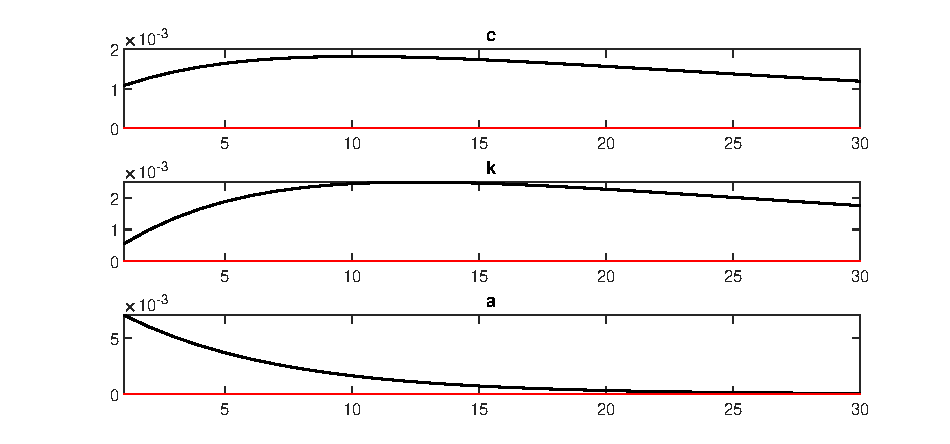
\includegraphics[width=\textwidth]{imgs/e_a.pdf} \label{fig irf}
\end{center}
\end{figure}%

%TCIMACRO{\TeXButton{BeginTable}{\begin{table}[h]
%\footnotesize}}%
%BeginExpansion
\begin{table}[h]
\footnotesize
%EndExpansion


\begin{center}%
\begin{tabular}
[c]{|l|l|}\hline
Stored in & Description\\\hline
\textit{oo\_} & Structure of the output of stoch\_simul function\\
oo\_.exo\_simul & Simulated series of the exogenous variables (if
simulating).\\
oo\_.endo\_simul & Simulated series of the endogenous variables (if
simulating).\\
oo\_.dr & Stored information about variables and policy function.\\
oo\_.dr.order\_var & The mapping from the declaration order to the decision
rule order.\\
oo\_.dr.inv\_order\_var & The mapping from the decision rule order to the
declaration order.\\
oo\_.dr.ghx & The A matrix of the transition function.\\
oo\_.dr.ghu & The B matrix of the transition function.\\
oo\_.steady\_state & Values of the endogenous variables' steady-state.\\
oo\_.gamma\_y & The variance decomposition outputted to the command window.\\
oo\_.mean & The mean of endogenous variables.\\
oo\_.var & The variance-covariance matrix.\\
oo\_.autocorr & The autocorrelation matrices for endogenous variables; up to 5
lags.\\
oo\_.irfs & Impulse responses of endogenous variables to exogenous shocks.\\
oo\_.irfs.x\_y & Impulse response of x to an innovation in y.\\
oo\_.forecast & Forecasts of endogenous variables.\\
& \\
\textit{M\_} & Structure with information about the model.\\
M\_.endo\_names & The names of endogenous variables in declaration order.\\
M\_.exo\_names & The names of exogenous variables in declaration order.\\
M\_.exo\_nbr & The number of exogenous variables.\\
M\_.endo\_nbr & The number of endogenous variables.\\
& \\
options\_ & Structure with all the options which Dynare recognises.\\\hline
\end{tabular}

\end{center}

%

%TCIMACRO{\TeXButton{titre du tableau - double cliquer pour editer}%
%{\caption{Matlab's workspace after a stochastic simulation \label
%{table workspace}}}}%
%BeginExpansion
\caption{Matlab's workspace after a stochastic simulation \label
{table workspace}}%
%EndExpansion%
%TCIMACRO{\TeXButton{EndTable}{\end{table}
%\normalsize\newpage}}%
%BeginExpansion
\end{table}
\normalsize\newpage
%EndExpansion


\newpage%
%TCIMACRO{\TeXButton{BeginExo}{\begin{myexercise}{extending the simple model}
%\addcontentsline{toc}{section}{Exercise \thetcbcounter}}}%
%BeginExpansion
\begin{myexercise}{extending the simple model}
\addcontentsline{toc}{section}{Exercise \thetcbcounter}%
%EndExpansion


Consider the file \textsf{basicRBC.mod}, the exercise aim at extending the model.

\begin{enumerate}
\item The GDP, $Y_{t}$ and investment $I_{t}$ are not (yet) included in the
model. Include them and draw their responses to a productivity shock. To do
so, log-linearize their equations and find their steady state.

\item Check whether the investment- to-gdp ratio $\bar{I}/\bar{Y}$ and
$\bar{C}/\bar{Y}$ are consistent with the data (on average, investment and
consumption represent respectively 20\%\ and 60\% of the GDP for
OECD\ countries). Why is there such a huge gap? How could you improve the RBC model?

\item Change the calibration to get a non-stationnary system response. What is
Dynare telling you in the command window? Does\ increasing return to scale
makes the model non-stationnary?
\end{enumerate}

%

%TCIMACRO{\TeXButton{EndExo}{\end{myexercise}}}%
%BeginExpansion
\end{myexercise}%
%EndExpansion


\newpage%

%TCIMACRO{\TeXButton{BeginExo}{\begin{myexercise}%
%{extension: habits in consumption}
%\addcontentsline{toc}{section}{Exercise \thetcbcounter}}}%
%BeginExpansion
\begin{myexercise}{extension: habits in consumption}
\addcontentsline{toc}{section}{Exercise \thetcbcounter}%
%EndExpansion


Theoretical macro models typically failed at reproducing the excess return
premium on financial markets before the 90s.\ In asset pricing theory, a new
consensus emerged to solve these puzzle through the inclusion of new
ingredients in macro-models which would help in solving the puzzle.\ One of
them is the consumption habits, pionereed by \cite{constantinides1990habit}
and \cite{abel1990asset}. Typically in real life situations, households have
strong consumption habits which materializes in time series by having a very
stable consumption over the business cycles, compared to other aggregates such
as investment and output. Basically, if the household decides the consume
more, it will raise the amount of consumption tomorrow. However, there is few
evidence about such behaviour at a micro-level, suggesting that consumption
habits is probably a shortcut for a more complex explanation of consumption inertia.

\begin{enumerate}
\item Let us assume first \textit{external} habits.\ These external habits
simply change how households are enjoying consumption in their utility
function:%
\begin{equation}
\mathcal{U}\left(  C_{jt}-hC_{t-1}\right)
\end{equation}
where $h\in\lbrack0,1)$\ is the degree of consumption habits. Here, it is
critical to notice that these habits are depending on the aggregate amount of
consumption $C_{t-1}$ (i.e. there is no subscript $j$). So basically, the
amount of aggregate consumption is not a control variable when households
maximizes utility. This is refered to as \textit{catching up with the jonese}
as people will copy the behaviour of the majority of consumers.\footnote{See
\cite{abel1990asset} the story about the Joneses.}

\begin{enumerate}
\item The marginal utility of consumption reads as : $\lambda_{t}%
=\mathcal{U}^{\prime}\left(  C_{jt}-hC_{t-1}\right)  $.

\item Find the steady state.

\item Linearize the expression. It might be useful to split the problem with
$\lambda_{t}=\mathcal{U}^{\prime}\left(  x_{t}\right)  $\ and $x_{t}%
=C_{t}-hC_{t-1}$ because the linearization trick cannot be applied for highly
non-linear problems.

\item How persistent is now consumption?
\end{enumerate}

\item Let us now assume internal habits, denoted $\mathcal{U}\left(
C_{jt}-hC_{jt-1}\right)  $.

\begin{enumerate}
\item The marginal utility of consumption reads as : $\lambda_{t}%
=\mathcal{U}^{\prime}\left(  C_{jt}-hC_{jt-1}\right)  -h\beta\mathcal{U}%
^{\prime}\left(  C_{jt+1}-hC_{t}\right)  $.

\item Find the steady state.

\item Linearize the expression. It might be useful to split again the problem
with $\lambda_{t}=\mathcal{U}^{\prime}\left(  x_{t}\right)  -\beta
h\mathcal{U}^{\prime}\left(  x_{t+1}\right)  $\ and $x_{t}=C_{t}-hC_{t-1}$.

\item How persistent is now consumption?
\end{enumerate}
\end{enumerate}

%

%TCIMACRO{\TeXButton{EndExo}{\end{myexercise}}}%
%BeginExpansion
\end{myexercise}%
%EndExpansion


\newpage%

%TCIMACRO{\TeXButton{BeginExo}{\begin{myexercise}{Demand shocks}
%\addcontentsline{toc}{section}{Exercise \thetcbcounter}}}%
%BeginExpansion
\begin{myexercise}{Demand shocks}
\addcontentsline{toc}{section}{Exercise \thetcbcounter}%
%EndExpansion


Assume now that our economy has a government.\ The government finances public
spending by charging a lump-sum tax $T_{jt}$\ on households.\ The total amount
of public spending reads as, $P_{t}G_{t}$. The balance sheet of government
writes:
\begin{equation}
P_{t}G_{t}=%
%TCIMACRO{\tint \nolimits_{0}^{1}}%
%BeginExpansion
{\textstyle\int\nolimits_{0}^{1}}
%EndExpansion
T_{jt}\text{d}j\text{ \ (=}T_{t}\text{)}.
\end{equation}
Since the economy is populated by an uniform household, we can write $T_{t}$
directly. The budget constraint of the representative household is now:%
\begin{equation}
C_{jt}+I_{jt}=A_{t}K_{jt-1}^{\alpha}-\frac{T_{jt}}{P_{t}},
\end{equation}
while the resource constraint/the GDP through the expenditure approach is now
given by:%
\begin{equation}
Y_{t}=C_{t}+I_{t}+G_{t}.
\end{equation}
The decision of increasing/decreasing spendings is decided exogenously by the
governement.\ In absence of an explicit modelling of political cycles, the
spending is assumed to vary around a fixed value of output:%
\begin{equation}
G_{t}=\bar{G}\varepsilon_{t}^{G}=g^{y}\bar{Y}\varepsilon_{t}^{G},
\end{equation}
where spending follows an $AR(1)$ process:%
\begin{equation}
\log\left(  \varepsilon_{t}^{G}\right)  =\rho_{G}\log\left(  \varepsilon
_{t-1}^{G}\right)  +\eta_{t}^{G},
\end{equation}
with $0\leq\rho_{G}<1$ is the autocorrelation coefficient of the demand shock
and $\eta_{t}^{G}$\ is an innovation distributed normally with zero mean and
finite variance $\sigma_{G}^{2}$ such that $\eta_{t}^{G}\sim\mathcal{N}%
(0,\sigma_{G}^{2})$. Parameter $g^{y}$ is the spending-to-GDP ratio. We borrow
the values of \cite{smets2007shocks}\ and assume that $\rho_{G}=0.97$,
$\sigma_{G}=0.053$ and $g^{y}=0.20$. Implicitely in steady state, the shock is
normalized to one $\bar{\varepsilon}^{G}=1$.

\begin{enumerate}
\item Compute the new steady state of the model. \textit{Tips:} (i) define a
new parameter, $g^{y}=0.2$, which affects the new steady state; (ii)\ since
the budget is balanced, you can substitute real taxes $T_{t}/P_{t}$ by
spending $G_{t}$.

\item Let's now calibrate the demand shock process, show the IRF after the
realization of the demand shock.

\item According to Keynesian economics, is this shock consistent with this
theory? Why do households are \textquotedblleft Ricardian\textquotedblright?
Is this behaviour observed in the data?

\item Analyse the variance decomposition, what is the main driver of output?

\item Is this RBC model now able to replicate another business cycle fact
which says output is more volatile than consumption?
\end{enumerate}

%

%TCIMACRO{\TeXButton{EndExo}{\end{myexercise}}}%
%BeginExpansion
\end{myexercise}%
%EndExpansion


\newpage%

%TCIMACRO{\TeXButton{small}{\footnotesize}}%
%BeginExpansion
\footnotesize
%EndExpansion
\bibliographystyle{plainnat}
\bibliography{dataref}%
%TCIMACRO{\TeXButton{small}{\normalsize}}%
%BeginExpansion
\normalsize
%EndExpansion



\end{document}
